% **************************************************************************************************
% **************************************************************************************************
\chapter{Appendix A}

In this appendix, we want to give the reader a better understanding of the timbre estimators' performance using the percussion, voice and e-guitar models as examples. For each of the three models, we produce a random mix (from the individual instrument tracks of a song), which contains the respective target instrument or family. Then we deploy the models to predict timbre descriptors and loudness of the target instrument or family and compare the prediction with the ground truth (=target).\footnote{Note: Do not confuse the \textit{target instrument} (or family) with the \textit{target} of a regression problem. Each model is trained to predict timbre descriptors of a particular target instrument (or family). The target, on the other hand, is the ground truth of these timbre descriptors.} Additionally, we report the \glspl{mae} between the predictions and the targets.
\section*{Percussion Model}
The audio mixture considered in this example contains a drum set, an electric bass and vocals of a standard pop song. The model's output and the corresponding targets are depicted in Fig.~\ref{fig:percussion-model}. 
\begin{figure}
	\captionsetup{list=no}
	\centering
	\subfigure[MFCCs]{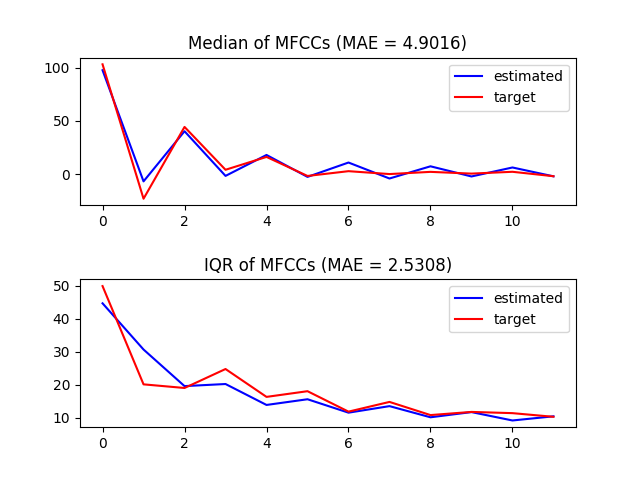
\includegraphics[width=0.52\textwidth]{appendix/figs/percussion-mfcc}}
	\subfigure[loudness and other timbre descriptors]{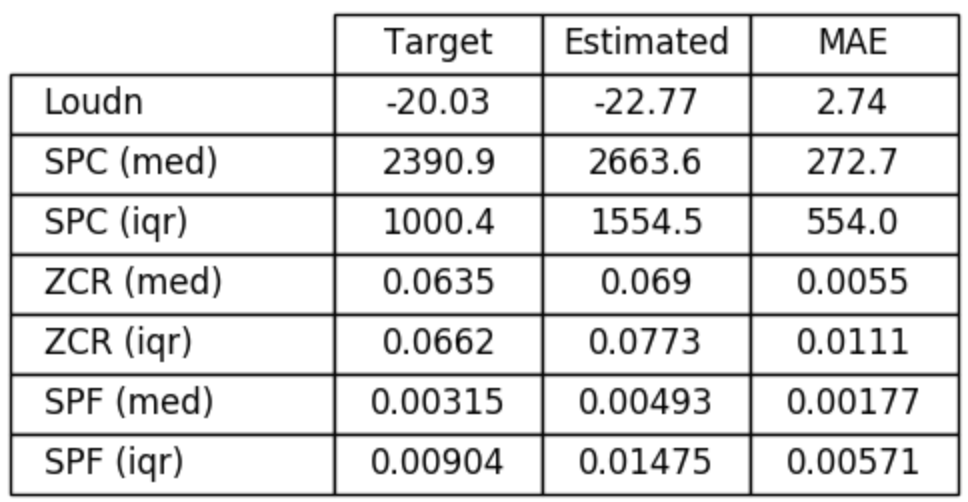
\includegraphics[width=0.42\textwidth, raise=0.6cm]{appendix/figs/percussion-descriptors}}
	\caption{Target and estimated timbre descriptors of a drum set in a pop song.}\label{fig:percussion-model}
\end{figure}
\section*{Voice Model}
In this example, the recording is a vanilla rock song with drum set, electric guitar, electric bass and (relatively quiet) vocals. The model's output and the corresponding targets are depicted in Fig.~\ref{fig:voice-model}.
\begin{figure}
	\captionsetup{list=no}
	\centering
	\subfigure[MFCCs]{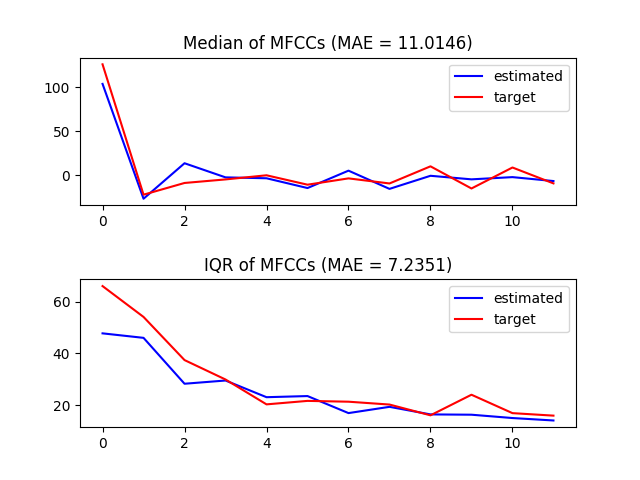
\includegraphics[width=0.52\textwidth]{appendix/figs/voice-mfcc}}
	\subfigure[loudness and other timbre descriptors]{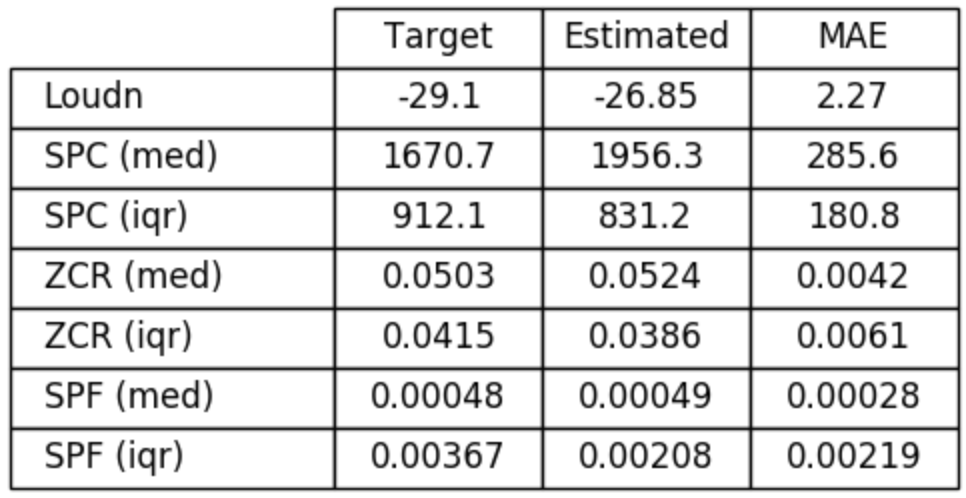
\includegraphics[width=0.42\textwidth, raise=0.6cm]{appendix/figs/voice-descriptors}}
	\caption{Target and estimated timbre descriptors of the vocals in a rock song.}\label{fig:voice-model}
\end{figure}
\section*{E-Guitar Model}
A metal song with drum set, highly distorted electric guitar and electric bass is used here. The model's output and the corresponding targets are depicted in Fig.~\ref{fig:e-guitar-model}.
\begin{figure}
	\captionsetup{list=no}
	\centering
	\subfigure[MFCCs]{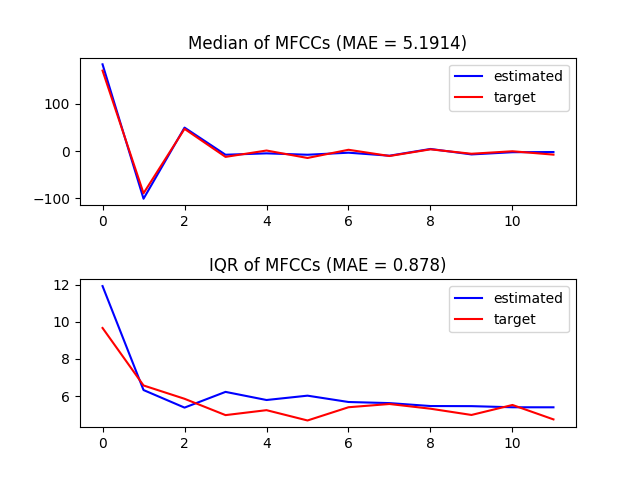
\includegraphics[width=0.52\textwidth]{appendix/figs/e-guitar-mfcc}}
	\subfigure[loudness and other timbre descriptors]{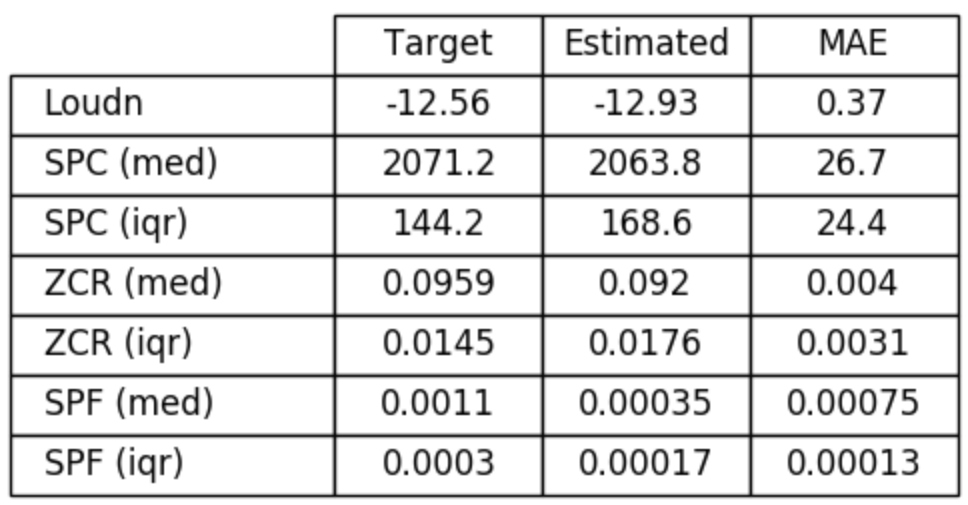
\includegraphics[width=0.42\textwidth, raise=0.6cm]{appendix/figs/e-guitar-descriptors}}
	\caption{Target and estimated timbre descriptors of the electric guitar in a metal song.}\label{fig:e-guitar-model}
\end{figure}\\

In general it can be said that the models, observed in the three examples above, perform exceptionally well at predicting timbre descriptors and loudness of the respective target instruments or families. Furthermore, although this is no surprise, we observe that the zero-crossing rate as well as the spectral centroid are larger for noisy sounds, like drum sets or distorted electric guitars, than for tonal sounds, such as vocals.





